\documentclass[1p]{elsarticle_modified}
%\bibliographystyle{elsarticle-num}

%\usepackage[colorlinks]{hyperref}
%\usepackage{abbrmath_seonhwa} %\Abb, \Ascr, \Acal ,\Abf, \Afrak
\usepackage{amsfonts}
\usepackage{amssymb}
\usepackage{amsmath}
\usepackage{amsthm}
\usepackage{scalefnt}
\usepackage{amsbsy}
\usepackage{kotex}
\usepackage{caption}
\usepackage{subfig}
\usepackage{color}
\usepackage{graphicx}
\usepackage{xcolor} %% white, black, red, green, blue, cyan, magenta, yellow
\usepackage{float}
\usepackage{setspace}
\usepackage{hyperref}

\usepackage{tikz}
\usetikzlibrary{arrows}

\usepackage{multirow}
\usepackage{array} % fixed length table
\usepackage{hhline}

%%%%%%%%%%%%%%%%%%%%%
\makeatletter
\renewcommand*\env@matrix[1][\arraystretch]{%
	\edef\arraystretch{#1}%
	\hskip -\arraycolsep
	\let\@ifnextchar\new@ifnextchar
	\array{*\c@MaxMatrixCols c}}
\makeatother %https://tex.stackexchange.com/questions/14071/how-can-i-increase-the-line-spacing-in-a-matrix
%%%%%%%%%%%%%%%

\usepackage[normalem]{ulem}

\newcommand{\msout}[1]{\ifmmode\text{\sout{\ensuremath{#1}}}\else\sout{#1}\fi}
%SOURCE: \msout is \stkout macro in https://tex.stackexchange.com/questions/20609/strikeout-in-math-mode

\newcommand{\cancel}[1]{
	\ifmmode
	{\color{red}\msout{#1}}
	\else
	{\color{red}\sout{#1}}
	\fi
}

\newcommand{\add}[1]{
	{\color{blue}\uwave{#1}}
}

\newcommand{\replace}[2]{
	\ifmmode
	{\color{red}\msout{#1}}{\color{blue}\uwave{#2}}
	\else
	{\color{red}\sout{#1}}{\color{blue}\uwave{#2}}
	\fi
}

\newcommand{\Sol}{\mathcal{S}} %segment
\newcommand{\D}{D} %diagram
\newcommand{\A}{\mathcal{A}} %arc


%%%%%%%%%%%%%%%%%%%%%%%%%%%%%5 test

\def\sl{\operatorname{\textup{SL}}(2,\Cbb)}
\def\psl{\operatorname{\textup{PSL}}(2,\Cbb)}
\def\quan{\mkern 1mu \triangleright \mkern 1mu}

\theoremstyle{definition}
\newtheorem{thm}{Theorem}[section]
\newtheorem{prop}[thm]{Proposition}
\newtheorem{lem}[thm]{Lemma}
\newtheorem{ques}[thm]{Question}
\newtheorem{cor}[thm]{Corollary}
\newtheorem{defn}[thm]{Definition}
\newtheorem{exam}[thm]{Example}
\newtheorem{rmk}[thm]{Remark}
\newtheorem{alg}[thm]{Algorithm}

\newcommand{\I}{\sqrt{-1}}
\begin{document}

%\begin{frontmatter}
%
%\title{Boundary parabolic representations of knots up to 8 crossings}
%
%%% Group authors per affiliation:
%\author{Yunhi Cho} 
%\address{Department of Mathematics, University of Seoul, Seoul, Korea}
%\ead{yhcho@uos.ac.kr}
%
%
%\author{Seonhwa Kim} %\fnref{s_kim}}
%\address{Center for Geometry and Physics, Institute for Basic Science, Pohang, 37673, Korea}
%\ead{ryeona17@ibs.re.kr}
%
%\author{Hyuk Kim}
%\address{Department of Mathematical Sciences, Seoul National University, Seoul 08826, Korea}
%\ead{hyukkim@snu.ac.kr}
%
%\author{Seokbeom Yoon}
%\address{Department of Mathematical Sciences, Seoul National University, Seoul, 08826,  Korea}
%\ead{sbyoon15@snu.ac.kr}
%
%\begin{abstract}
%We find all boundary parabolic representation of knots up to 8 crossings.
%
%\end{abstract}
%\begin{keyword}
%    \MSC[2010] 57M25 
%\end{keyword}
%
%\end{frontmatter}

%\linenumbers
%\tableofcontents
%
\newcommand\colored[1]{\textcolor{white}{\rule[-0.35ex]{0.8em}{1.4ex}}\kern-0.8em\color{red} #1}%
%\newcommand\colored[1]{\textcolor{white}{ #1}\kern-2.17ex	\textcolor{white}{ #1}\kern-1.81ex	\textcolor{white}{ #1}\kern-2.15ex\color{red}#1	}

{\Large $\underline{12a_{1185}~(K12a_{1185})}$}

\setlength{\tabcolsep}{10pt}
\renewcommand{\arraystretch}{1.6}
\vspace{1cm}\begin{tabular}{m{100pt}>{\centering\arraybackslash}m{274pt}}
\multirow{5}{120pt}{
	\centering
	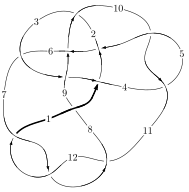
\includegraphics[width=112pt]{../../../GIT/diagram.site/Diagrams/png/1986_12a_1185.png}\\
\ \ \ A knot diagram\footnotemark}&
\allowdisplaybreaks
\textbf{Linearized knot diagam} \\
\cline{2-2}
 &
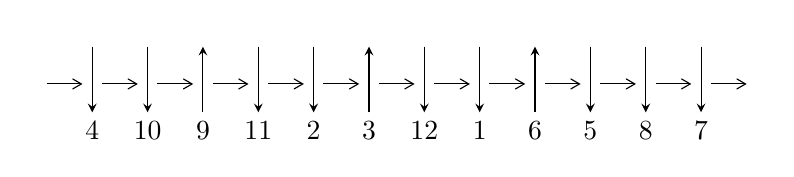
\begin{tikzpicture}[x=20pt, y=17pt]
	% nodes
	\node (C0) at (0, 0) {};
	\node (C1) at (1, 0) {};
	\node (C1U) at (1, +1) {};
	\node (C1D) at (1, -1) {4};

	\node (C2) at (2, 0) {};
	\node (C2U) at (2, +1) {};
	\node (C2D) at (2, -1) {10};

	\node (C3) at (3, 0) {};
	\node (C3U) at (3, +1) {};
	\node (C3D) at (3, -1) {9};

	\node (C4) at (4, 0) {};
	\node (C4U) at (4, +1) {};
	\node (C4D) at (4, -1) {11};

	\node (C5) at (5, 0) {};
	\node (C5U) at (5, +1) {};
	\node (C5D) at (5, -1) {2};

	\node (C6) at (6, 0) {};
	\node (C6U) at (6, +1) {};
	\node (C6D) at (6, -1) {3};

	\node (C7) at (7, 0) {};
	\node (C7U) at (7, +1) {};
	\node (C7D) at (7, -1) {12};

	\node (C8) at (8, 0) {};
	\node (C8U) at (8, +1) {};
	\node (C8D) at (8, -1) {1};

	\node (C9) at (9, 0) {};
	\node (C9U) at (9, +1) {};
	\node (C9D) at (9, -1) {6};

	\node (C10) at (10, 0) {};
	\node (C10U) at (10, +1) {};
	\node (C10D) at (10, -1) {5};

	\node (C11) at (11, 0) {};
	\node (C11U) at (11, +1) {};
	\node (C11D) at (11, -1) {8};

	\node (C12) at (12, 0) {};
	\node (C12U) at (12, +1) {};
	\node (C12D) at (12, -1) {7};
	\node (C13) at (13, 0) {};

	% arrows
	\draw[->,>={angle 60}]
	(C0) edge (C1) (C1) edge (C2) (C2) edge (C3) (C3) edge (C4) (C4) edge (C5) (C5) edge (C6) (C6) edge (C7) (C7) edge (C8) (C8) edge (C9) (C9) edge (C10) (C10) edge (C11) (C11) edge (C12) (C12) edge (C13) ;	\draw[->,>=stealth]
	(C1U) edge (C1D) (C2U) edge (C2D) (C3D) edge (C3U) (C4U) edge (C4D) (C5U) edge (C5D) (C6D) edge (C6U) (C7U) edge (C7D) (C8U) edge (C8D) (C9D) edge (C9U) (C10U) edge (C10D) (C11U) edge (C11D) (C12U) edge (C12D) ;
	\end{tikzpicture} \\
\hhline{~~} \\& 
\textbf{Solving Sequence} \\ \cline{2-2} 
 &
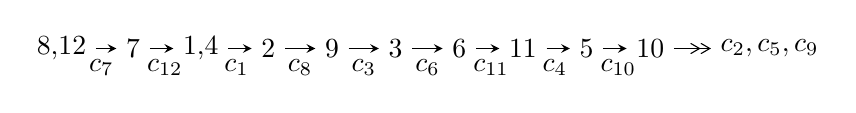
\begin{tikzpicture}[x=23pt, y=7pt]
	% node
	\node (A0) at (-1/8, 0) {8,12};
	\node (A1) at (1, 0) {7};
	\node (A2) at (33/16, 0) {1,4};
	\node (A3) at (25/8, 0) {2};
	\node (A4) at (33/8, 0) {9};
	\node (A5) at (41/8, 0) {3};
	\node (A6) at (49/8, 0) {6};
	\node (A7) at (57/8, 0) {11};
	\node (A8) at (65/8, 0) {5};
	\node (A9) at (73/8, 0) {10};
	\node (C1) at (1/2, -1) {$c_{7}$};
	\node (C2) at (3/2, -1) {$c_{12}$};
	\node (C3) at (21/8, -1) {$c_{1}$};
	\node (C4) at (29/8, -1) {$c_{8}$};
	\node (C5) at (37/8, -1) {$c_{3}$};
	\node (C6) at (45/8, -1) {$c_{6}$};
	\node (C7) at (53/8, -1) {$c_{11}$};
	\node (C8) at (61/8, -1) {$c_{4}$};
	\node (C9) at (69/8, -1) {$c_{10}$};
	\node (A10) at (11, 0) {$c_{2},c_{5},c_{9}$};

	% edge
	\draw[->,>=stealth]	
	(A0) edge (A1) (A1) edge (A2) (A2) edge (A3) (A3) edge (A4) (A4) edge (A5) (A5) edge (A6) (A6) edge (A7) (A7) edge (A8) (A8) edge (A9) ;
	\draw[->>,>={angle 60}]	
	(A9) edge (A10);
\end{tikzpicture} \\ 

\end{tabular} \\

\footnotetext{
The image of knot diagram is generated by the software ``\textbf{Draw programme}" developed by Andrew Bartholomew(\url{http://www.layer8.co.uk/maths/draw/index.htm\#Running-draw}), where we modified some parts for our purpose(\url{https://github.com/CATsTAILs/LinksPainter}).
}\phantom \\ \newline 
\centering \textbf{Ideals for irreducible components\footnotemark of $X_{\text{par}}$} 
 
\begin{align*}
I^u_{1}&=\langle 
1.11343\times10^{206} u^{141}+7.40241\times10^{206} u^{140}+\cdots+6.56549\times10^{206} b+6.12514\times10^{208},\\
\phantom{I^u_{1}}&\phantom{= \langle  }-3.17039\times10^{208} u^{141}+3.40884\times10^{208} u^{140}+\cdots+1.24744\times10^{208} a-7.01718\times10^{209},\\
\phantom{I^u_{1}}&\phantom{= \langle  }u^{142}+65 u^{140}+\cdots+79 u+19\rangle \\
I^u_{2}&=\langle 
-4 u^{24}+2 u^{23}+\cdots+b+3,\;-16 u^{24}-7 u^{23}+\cdots+a+47,\;u^{25}+u^{24}+\cdots-4 u-1\rangle \\
\\
\end{align*}
\raggedright * 2 irreducible components of $\dim_{\mathbb{C}}=0$, with total 167 representations.\\
\footnotetext{All coefficients of polynomials are rational numbers. But the coefficients are sometimes approximated in decimal forms when there is not enough margin.}
\newpage
\renewcommand{\arraystretch}{1}
\centering \section*{I. $I^u_{1}= \langle 1.11\times10^{206} u^{141}+7.40\times10^{206} u^{140}+\cdots+6.57\times10^{206} b+6.13\times10^{208},\;-3.17\times10^{208} u^{141}+3.41\times10^{208} u^{140}+\cdots+1.25\times10^{208} a-7.02\times10^{209},\;u^{142}+65 u^{140}+\cdots+79 u+19 \rangle$}
\flushleft \textbf{(i) Arc colorings}\\
\begin{tabular}{m{7pt} m{180pt} m{7pt} m{180pt} }
\flushright $a_{8}=$&$\begin{pmatrix}1\\0\end{pmatrix}$ \\
\flushright $a_{12}=$&$\begin{pmatrix}0\\u\end{pmatrix}$ \\
\flushright $a_{7}=$&$\begin{pmatrix}1\\- u^2\end{pmatrix}$ \\
\flushright $a_{1}=$&$\begin{pmatrix}- u\\u^3+u\end{pmatrix}$ \\
\flushright $a_{4}=$&$\begin{pmatrix}2.54151 u^{141}-2.73266 u^{140}+\cdots+76.5272 u+56.2525\\-0.169589 u^{141}-1.12747 u^{140}+\cdots-204.010 u-93.2930\end{pmatrix}$ \\
\flushright $a_{2}=$&$\begin{pmatrix}-2.43322 u^{141}+2.31831 u^{140}+\cdots-72.4795 u-23.3362\\-1.75719 u^{141}+2.11532 u^{140}+\cdots-21.2865 u-16.5595\end{pmatrix}$ \\
\flushright $a_{9}=$&$\begin{pmatrix}- u^4- u^2+1\\u^6+2 u^4+u^2\end{pmatrix}$ \\
\flushright $a_{3}=$&$\begin{pmatrix}4.10649 u^{141}-2.52027 u^{140}+\cdots+221.136 u+119.028\\0.548199 u^{141}-0.503020 u^{140}+\cdots-122.486 u-62.6947\end{pmatrix}$ \\
\flushright $a_{6}=$&$\begin{pmatrix}-0.928942 u^{141}+1.82621 u^{140}+\cdots+99.1463 u+52.5504\\-3.13792 u^{141}+2.98162 u^{140}+\cdots-61.4178 u-37.8642\end{pmatrix}$ \\
\flushright $a_{11}=$&$\begin{pmatrix}u\\u\end{pmatrix}$ \\
\flushright $a_{5}=$&$\begin{pmatrix}4.82524 u^{141}-3.49571 u^{140}+\cdots+151.827 u+86.7511\\2.11414 u^{141}-1.89052 u^{140}+\cdots-128.710 u-62.7943\end{pmatrix}$ \\
\flushright $a_{10}=$&$\begin{pmatrix}8.26655 u^{141}-4.17721 u^{140}+\cdots+448.015 u+186.893\\2.46556 u^{141}-2.77177 u^{140}+\cdots-192.455 u-99.7949\end{pmatrix}$\\&\end{tabular}
\flushleft \textbf{(ii) Obstruction class $= -1$}\\~\\
\flushleft \textbf{(iii) Cusp Shapes $= 198.235 u^{141}-76.2003 u^{140}+\cdots+18676.8 u+8619.47$}\\~\\
\newpage\renewcommand{\arraystretch}{1}
\flushleft \textbf{(iv) u-Polynomials at the component}\newline \\
\begin{tabular}{m{50pt}|m{274pt}}
Crossings & \hspace{64pt}u-Polynomials at each crossing \\
\hline $$\begin{aligned}c_{1}\end{aligned}$$&$\begin{aligned}
&u^{142}+3 u^{141}+\cdots+25660 u+1552
\end{aligned}$\\
\hline $$\begin{aligned}c_{2}\end{aligned}$$&$\begin{aligned}
&u^{142}-3 u^{141}+\cdots+3363 u-9621
\end{aligned}$\\
\hline $$\begin{aligned}c_{3}\end{aligned}$$&$\begin{aligned}
&u^{142}- u^{141}+\cdots+20522 u-1087
\end{aligned}$\\
\hline $$\begin{aligned}c_{4},c_{10}\end{aligned}$$&$\begin{aligned}
&u^{142}- u^{141}+\cdots-39669 u-8231
\end{aligned}$\\
\hline $$\begin{aligned}c_{5}\end{aligned}$$&$\begin{aligned}
&u^{142}-2 u^{141}+\cdots-22 u+1
\end{aligned}$\\
\hline $$\begin{aligned}c_{6}\end{aligned}$$&$\begin{aligned}
&u^{142}-4 u^{141}+\cdots-13583 u-2209
\end{aligned}$\\
\hline $$\begin{aligned}c_{7},c_{11},c_{12}\end{aligned}$$&$\begin{aligned}
&u^{142}+65 u^{140}+\cdots+79 u+19
\end{aligned}$\\
\hline $$\begin{aligned}c_{8}\end{aligned}$$&$\begin{aligned}
&u^{142}-5 u^{139}+\cdots-918747 u+290111
\end{aligned}$\\
\hline $$\begin{aligned}c_{9}\end{aligned}$$&$\begin{aligned}
&u^{142}-5 u^{141}+\cdots-30 u-4
\end{aligned}$\\
\hline
\end{tabular}\\~\\
\newpage\renewcommand{\arraystretch}{1}
\flushleft \textbf{(v) Riley Polynomials at the component}\newline \\
\begin{tabular}{m{50pt}|m{274pt}}
Crossings & \hspace{64pt}Riley Polynomials at each crossing \\
\hline $$\begin{aligned}c_{1}\end{aligned}$$&$\begin{aligned}
&y^{142}+9 y^{141}+\cdots-198506608 y+2408704
\end{aligned}$\\
\hline $$\begin{aligned}c_{2}\end{aligned}$$&$\begin{aligned}
&y^{142}+33 y^{141}+\cdots+5619168819 y+92563641
\end{aligned}$\\
\hline $$\begin{aligned}c_{3}\end{aligned}$$&$\begin{aligned}
&y^{142}+7 y^{141}+\cdots-23640932 y+1181569
\end{aligned}$\\
\hline $$\begin{aligned}c_{4},c_{10}\end{aligned}$$&$\begin{aligned}
&y^{142}+91 y^{141}+\cdots+2568604727 y+67749361
\end{aligned}$\\
\hline $$\begin{aligned}c_{5}\end{aligned}$$&$\begin{aligned}
&y^{142}+22 y^{141}+\cdots-108 y+1
\end{aligned}$\\
\hline $$\begin{aligned}c_{6}\end{aligned}$$&$\begin{aligned}
&y^{142}-8 y^{141}+\cdots-159226929 y+4879681
\end{aligned}$\\
\hline $$\begin{aligned}c_{7},c_{11},c_{12}\end{aligned}$$&$\begin{aligned}
&y^{142}+130 y^{141}+\cdots-3391 y+361
\end{aligned}$\\
\hline $$\begin{aligned}c_{8}\end{aligned}$$&$\begin{aligned}
&y^{142}+48 y^{140}+\cdots+676166821071 y+84164392321
\end{aligned}$\\
\hline $$\begin{aligned}c_{9}\end{aligned}$$&$\begin{aligned}
&y^{142}+y^{141}+\cdots+308 y+16
\end{aligned}$\\
\hline
\end{tabular}\\~\\
\newpage\flushleft \textbf{(vi) Complex Volumes and Cusp Shapes}
$$\begin{array}{c|c|c}  
\text{Solutions to }I^u_{1}& \I (\text{vol} + \sqrt{-1}CS) & \text{Cusp shape}\\
 \hline 
\begin{aligned}
u &= -0.174055 + 0.972792 I \\
a &= \phantom{-}1.13546 + 1.26631 I \\
b &= \phantom{-}0.213062 + 1.135370 I\end{aligned}
 & \phantom{-}0.15417 + 3.00552 I & \phantom{-0.000000 } 0 \\ \hline\begin{aligned}
u &= -0.174055 - 0.972792 I \\
a &= \phantom{-}1.13546 - 1.26631 I \\
b &= \phantom{-}0.213062 - 1.135370 I\end{aligned}
 & \phantom{-}0.15417 - 3.00552 I & \phantom{-0.000000 } 0 \\ \hline\begin{aligned}
u &= -0.576373 + 0.859061 I \\
a &= -0.899351 + 0.405170 I \\
b &= -0.043856 - 0.230883 I\end{aligned}
 & \phantom{-}3.29168 - 0.88987 I & \phantom{-0.000000 } 0 \\ \hline\begin{aligned}
u &= -0.576373 - 0.859061 I \\
a &= -0.899351 - 0.405170 I \\
b &= -0.043856 + 0.230883 I\end{aligned}
 & \phantom{-}3.29168 + 0.88987 I & \phantom{-0.000000 } 0 \\ \hline\begin{aligned}
u &= -0.356081 + 0.885492 I \\
a &= \phantom{-}0.090876 - 1.372330 I \\
b &= \phantom{-}0.234041 - 0.386315 I\end{aligned}
 & -1.57123 + 4.66450 I & \phantom{-0.000000 } 0 \\ \hline\begin{aligned}
u &= -0.356081 - 0.885492 I \\
a &= \phantom{-}0.090876 + 1.372330 I \\
b &= \phantom{-}0.234041 + 0.386315 I\end{aligned}
 & -1.57123 - 4.66450 I & \phantom{-0.000000 } 0 \\ \hline\begin{aligned}
u &= \phantom{-}0.337165 + 0.880232 I \\
a &= -0.44299 - 1.50054 I \\
b &= -0.847248 - 0.424499 I\end{aligned}
 & -1.57542 + 5.20147 I & \phantom{-0.000000 } 0 \\ \hline\begin{aligned}
u &= \phantom{-}0.337165 - 0.880232 I \\
a &= -0.44299 + 1.50054 I \\
b &= -0.847248 + 0.424499 I\end{aligned}
 & -1.57542 - 5.20147 I & \phantom{-0.000000 } 0 \\ \hline\begin{aligned}
u &= -0.511808 + 0.786498 I \\
a &= \phantom{-}1.21144 - 1.10273 I \\
b &= \phantom{-}0.292622 + 0.143049 I\end{aligned}
 & \phantom{-}2.74351 - 10.79950 I & \phantom{-0.000000 } 0 \\ \hline\begin{aligned}
u &= -0.511808 - 0.786498 I \\
a &= \phantom{-}1.21144 + 1.10273 I \\
b &= \phantom{-}0.292622 - 0.143049 I\end{aligned}
 & \phantom{-}2.74351 + 10.79950 I & \phantom{-0.000000 } 0\\
 \hline 
 \end{array}$$\newpage$$\begin{array}{c|c|c}  
\text{Solutions to }I^u_{1}& \I (\text{vol} + \sqrt{-1}CS) & \text{Cusp shape}\\
 \hline 
\begin{aligned}
u &= \phantom{-}0.533098 + 0.756555 I \\
a &= -0.943932 - 0.943336 I \\
b &= -0.172542 + 0.320177 I\end{aligned}
 & \phantom{-}4.17740 + 2.66753 I & \phantom{-0.000000 } 0 \\ \hline\begin{aligned}
u &= \phantom{-}0.533098 - 0.756555 I \\
a &= -0.943932 + 0.943336 I \\
b &= -0.172542 - 0.320177 I\end{aligned}
 & \phantom{-}4.17740 - 2.66753 I & \phantom{-0.000000 } 0 \\ \hline\begin{aligned}
u &= -0.841285 + 0.306784 I \\
a &= \phantom{-}0.213661 + 0.256949 I \\
b &= \phantom{-}0.804634 - 0.897367 I\end{aligned}
 & \phantom{-}1.57602 + 5.81227 I & \phantom{-0.000000 } 0 \\ \hline\begin{aligned}
u &= -0.841285 - 0.306784 I \\
a &= \phantom{-}0.213661 - 0.256949 I \\
b &= \phantom{-}0.804634 + 0.897367 I\end{aligned}
 & \phantom{-}1.57602 - 5.81227 I & \phantom{-0.000000 } 0 \\ \hline\begin{aligned}
u &= -0.345187 + 1.051640 I \\
a &= -1.67103 + 0.42473 I \\
b &= -0.713812 - 0.123338 I\end{aligned}
 & \phantom{-}1.77024 - 1.80840 I & \phantom{-0.000000 } 0 \\ \hline\begin{aligned}
u &= -0.345187 - 1.051640 I \\
a &= -1.67103 - 0.42473 I \\
b &= -0.713812 + 0.123338 I\end{aligned}
 & \phantom{-}1.77024 + 1.80840 I & \phantom{-0.000000 } 0 \\ \hline\begin{aligned}
u &= -0.068764 + 1.137420 I \\
a &= -0.06703 + 2.34760 I \\
b &= -0.65565 + 1.99120 I\end{aligned}
 & -0.781789 + 0.146833 I & \phantom{-0.000000 } 0 \\ \hline\begin{aligned}
u &= -0.068764 - 1.137420 I \\
a &= -0.06703 - 2.34760 I \\
b &= -0.65565 - 1.99120 I\end{aligned}
 & -0.781789 - 0.146833 I & \phantom{-0.000000 } 0 \\ \hline\begin{aligned}
u &= -0.795014 + 0.304336 I \\
a &= -0.230248 - 0.310817 I \\
b &= -1.42055 + 1.02178 I\end{aligned}
 & \phantom{-}1.1763 + 15.3660 I & \phantom{-0.000000 } 0 \\ \hline\begin{aligned}
u &= -0.795014 - 0.304336 I \\
a &= -0.230248 + 0.310817 I \\
b &= -1.42055 - 1.02178 I\end{aligned}
 & \phantom{-}1.1763 - 15.3660 I & \phantom{-0.000000 } 0\\
 \hline 
 \end{array}$$\newpage$$\begin{array}{c|c|c}  
\text{Solutions to }I^u_{1}& \I (\text{vol} + \sqrt{-1}CS) & \text{Cusp shape}\\
 \hline 
\begin{aligned}
u &= \phantom{-}0.786923 + 0.312206 I \\
a &= \phantom{-}0.018638 - 0.341669 I \\
b &= \phantom{-}1.27663 + 0.91277 I\end{aligned}
 & \phantom{-}2.72275 - 7.22715 I & \phantom{-0.000000 } 0 \\ \hline\begin{aligned}
u &= \phantom{-}0.786923 - 0.312206 I \\
a &= \phantom{-}0.018638 + 0.341669 I \\
b &= \phantom{-}1.27663 - 0.91277 I\end{aligned}
 & \phantom{-}2.72275 + 7.22715 I & \phantom{-0.000000 } 0 \\ \hline\begin{aligned}
u &= \phantom{-}0.844094 + 0.041958 I \\
a &= \phantom{-}0.040538 + 0.442418 I \\
b &= \phantom{-}0.519571 - 0.757023 I\end{aligned}
 & -2.06705 + 5.32893 I & \phantom{-0.000000 } 0 \\ \hline\begin{aligned}
u &= \phantom{-}0.844094 - 0.041958 I \\
a &= \phantom{-}0.040538 - 0.442418 I \\
b &= \phantom{-}0.519571 + 0.757023 I\end{aligned}
 & -2.06705 - 5.32893 I & \phantom{-0.000000 } 0 \\ \hline\begin{aligned}
u &= -0.782943 + 0.220151 I \\
a &= \phantom{-}0.013266 - 0.208503 I \\
b &= -1.158200 + 0.084694 I\end{aligned}
 & -3.70212 - 0.47486 I & \phantom{-0.000000 } 0 \\ \hline\begin{aligned}
u &= -0.782943 - 0.220151 I \\
a &= \phantom{-}0.013266 + 0.208503 I \\
b &= -1.158200 - 0.084694 I\end{aligned}
 & -3.70212 + 0.47486 I & \phantom{-0.000000 } 0 \\ \hline\begin{aligned}
u &= \phantom{-}0.235609 + 1.170740 I \\
a &= \phantom{-}0.130480 - 0.364998 I \\
b &= \phantom{-}0.390627 + 0.025420 I\end{aligned}
 & \phantom{-}1.54848 + 0.94593 I & \phantom{-0.000000 } 0 \\ \hline\begin{aligned}
u &= \phantom{-}0.235609 - 1.170740 I \\
a &= \phantom{-}0.130480 + 0.364998 I \\
b &= \phantom{-}0.390627 - 0.025420 I\end{aligned}
 & \phantom{-}1.54848 - 0.94593 I & \phantom{-0.000000 } 0 \\ \hline\begin{aligned}
u &= \phantom{-}0.412086 + 1.126510 I \\
a &= \phantom{-}0.461038 - 1.157240 I \\
b &= -0.582522 - 1.088710 I\end{aligned}
 & \phantom{-}1.26907 - 9.81961 I & \phantom{-0.000000 } 0 \\ \hline\begin{aligned}
u &= \phantom{-}0.412086 - 1.126510 I \\
a &= \phantom{-}0.461038 + 1.157240 I \\
b &= -0.582522 + 1.088710 I\end{aligned}
 & \phantom{-}1.26907 + 9.81961 I & \phantom{-0.000000 } 0\\
 \hline 
 \end{array}$$\newpage$$\begin{array}{c|c|c}  
\text{Solutions to }I^u_{1}& \I (\text{vol} + \sqrt{-1}CS) & \text{Cusp shape}\\
 \hline 
\begin{aligned}
u &= -0.254377 + 1.176850 I \\
a &= \phantom{-}0.003247 - 1.401810 I \\
b &= \phantom{-}0.773222 - 0.895144 I\end{aligned}
 & \phantom{-}2.22220 + 2.62980 I & \phantom{-0.000000 } 0 \\ \hline\begin{aligned}
u &= -0.254377 - 1.176850 I \\
a &= \phantom{-}0.003247 + 1.401810 I \\
b &= \phantom{-}0.773222 + 0.895144 I\end{aligned}
 & \phantom{-}2.22220 - 2.62980 I & \phantom{-0.000000 } 0 \\ \hline\begin{aligned}
u &= \phantom{-}0.219631 + 1.185970 I \\
a &= \phantom{-}1.04945 + 1.66768 I \\
b &= \phantom{-}1.30300 + 1.28806 I\end{aligned}
 & -1.29585 - 1.11745 I & \phantom{-0.000000 } 0 \\ \hline\begin{aligned}
u &= \phantom{-}0.219631 - 1.185970 I \\
a &= \phantom{-}1.04945 - 1.66768 I \\
b &= \phantom{-}1.30300 - 1.28806 I\end{aligned}
 & -1.29585 + 1.11745 I & \phantom{-0.000000 } 0 \\ \hline\begin{aligned}
u &= \phantom{-}0.759399 + 0.228128 I \\
a &= \phantom{-}0.022365 + 0.314814 I \\
b &= \phantom{-}1.53675 + 0.03121 I\end{aligned}
 & -3.65601 - 9.26795 I & \phantom{-0.000000 } 0 \\ \hline\begin{aligned}
u &= \phantom{-}0.759399 - 0.228128 I \\
a &= \phantom{-}0.022365 - 0.314814 I \\
b &= \phantom{-}1.53675 - 0.03121 I\end{aligned}
 & -3.65601 + 9.26795 I & \phantom{-0.000000 } 0 \\ \hline\begin{aligned}
u &= -0.761357 + 0.167439 I \\
a &= \phantom{-}0.447181 + 0.166476 I \\
b &= \phantom{-}1.19140 - 1.30202 I\end{aligned}
 & -0.90067 + 5.85726 I & \phantom{-0.000000 } 0 \\ \hline\begin{aligned}
u &= -0.761357 - 0.167439 I \\
a &= \phantom{-}0.447181 - 0.166476 I \\
b &= \phantom{-}1.19140 + 1.30202 I\end{aligned}
 & -0.90067 - 5.85726 I & \phantom{-0.000000 } 0 \\ \hline\begin{aligned}
u &= \phantom{-}0.409078 + 1.164650 I \\
a &= -0.442972 + 0.154483 I \\
b &= \phantom{-}0.137302 + 0.558531 I\end{aligned}
 & \phantom{-}1.71521 + 0.89999 I & \phantom{-0.000000 } 0 \\ \hline\begin{aligned}
u &= \phantom{-}0.409078 - 1.164650 I \\
a &= -0.442972 - 0.154483 I \\
b &= \phantom{-}0.137302 - 0.558531 I\end{aligned}
 & \phantom{-}1.71521 - 0.89999 I & \phantom{-0.000000 } 0\\
 \hline 
 \end{array}$$\newpage$$\begin{array}{c|c|c}  
\text{Solutions to }I^u_{1}& \I (\text{vol} + \sqrt{-1}CS) & \text{Cusp shape}\\
 \hline 
\begin{aligned}
u &= \phantom{-}0.645504 + 0.408312 I \\
a &= -0.209626 + 0.955204 I \\
b &= -0.996395 - 0.051955 I\end{aligned}
 & -1.63352 - 2.00241 I & \phantom{-0.000000 } 0 \\ \hline\begin{aligned}
u &= \phantom{-}0.645504 - 0.408312 I \\
a &= -0.209626 - 0.955204 I \\
b &= -0.996395 + 0.051955 I\end{aligned}
 & -1.63352 + 2.00241 I & \phantom{-0.000000 } 0 \\ \hline\begin{aligned}
u &= \phantom{-}0.265669 + 0.715458 I \\
a &= \phantom{-}1.51827 + 1.21207 I \\
b &= \phantom{-}0.438576 + 0.389675 I\end{aligned}
 & \phantom{-}0.36527 + 2.98078 I & \phantom{-0.000000 } 0 \\ \hline\begin{aligned}
u &= \phantom{-}0.265669 - 0.715458 I \\
a &= \phantom{-}1.51827 - 1.21207 I \\
b &= \phantom{-}0.438576 - 0.389675 I\end{aligned}
 & \phantom{-}0.36527 - 2.98078 I & \phantom{-0.000000 } 0 \\ \hline\begin{aligned}
u &= \phantom{-}0.717874 + 0.255264 I \\
a &= -0.522373 + 0.071194 I \\
b &= -1.46414 - 1.04875 I\end{aligned}
 & -1.33895 - 6.73506 I & \phantom{-0.000000 } 0 \\ \hline\begin{aligned}
u &= \phantom{-}0.717874 - 0.255264 I \\
a &= -0.522373 - 0.071194 I \\
b &= -1.46414 + 1.04875 I\end{aligned}
 & -1.33895 + 6.73506 I & \phantom{-0.000000 } 0 \\ \hline\begin{aligned}
u &= -0.014781 + 1.250720 I \\
a &= \phantom{-}2.43752 + 0.18416 I \\
b &= \phantom{-}1.71375 - 0.16619 I\end{aligned}
 & \phantom{-}5.81117 + 5.18320 I & \phantom{-0.000000 } 0 \\ \hline\begin{aligned}
u &= -0.014781 - 1.250720 I \\
a &= \phantom{-}2.43752 - 0.18416 I \\
b &= \phantom{-}1.71375 + 0.16619 I\end{aligned}
 & \phantom{-}5.81117 - 5.18320 I & \phantom{-0.000000 } 0 \\ \hline\begin{aligned}
u &= \phantom{-}0.724193 + 0.178608 I \\
a &= -0.295872 - 0.572436 I \\
b &= -0.325525 - 0.319339 I\end{aligned}
 & -1.22360 - 4.51757 I & \phantom{-0.000000 } 0 \\ \hline\begin{aligned}
u &= \phantom{-}0.724193 - 0.178608 I \\
a &= -0.295872 + 0.572436 I \\
b &= -0.325525 + 0.319339 I\end{aligned}
 & -1.22360 + 4.51757 I & \phantom{-0.000000 } 0\\
 \hline 
 \end{array}$$\newpage$$\begin{array}{c|c|c}  
\text{Solutions to }I^u_{1}& \I (\text{vol} + \sqrt{-1}CS) & \text{Cusp shape}\\
 \hline 
\begin{aligned}
u &= \phantom{-}0.532726 + 0.503092 I \\
a &= -0.973548 - 0.549870 I \\
b &= \phantom{-}0.286092 + 0.678139 I\end{aligned}
 & \phantom{-}3.43249 - 1.96165 I & \phantom{-0.000000 } 0 \\ \hline\begin{aligned}
u &= \phantom{-}0.532726 - 0.503092 I \\
a &= -0.973548 + 0.549870 I \\
b &= \phantom{-}0.286092 - 0.678139 I\end{aligned}
 & \phantom{-}3.43249 + 1.96165 I & \phantom{-0.000000 } 0 \\ \hline\begin{aligned}
u &= -0.147133 + 1.276140 I \\
a &= -1.44340 - 0.15442 I \\
b &= -0.230016 - 0.523489 I\end{aligned}
 & \phantom{-}4.66589 + 1.67554 I & \phantom{-0.000000 } 0 \\ \hline\begin{aligned}
u &= -0.147133 - 1.276140 I \\
a &= -1.44340 + 0.15442 I \\
b &= -0.230016 + 0.523489 I\end{aligned}
 & \phantom{-}4.66589 - 1.67554 I & \phantom{-0.000000 } 0 \\ \hline\begin{aligned}
u &= -0.684540 + 0.197429 I \\
a &= \phantom{-}0.366121 - 0.249618 I \\
b &= \phantom{-}0.387064 + 0.757529 I\end{aligned}
 & -2.15344 + 0.42861 I & \phantom{-0.000000 } 0 \\ \hline\begin{aligned}
u &= -0.684540 - 0.197429 I \\
a &= \phantom{-}0.366121 + 0.249618 I \\
b &= \phantom{-}0.387064 - 0.757529 I\end{aligned}
 & -2.15344 - 0.42861 I & \phantom{-0.000000 } 0 \\ \hline\begin{aligned}
u &= -0.124470 + 1.301350 I \\
a &= -1.19386 - 1.16644 I \\
b &= -2.22445 - 0.90074 I\end{aligned}
 & \phantom{-}6.87784 - 3.48818 I & \phantom{-0.000000 } 0 \\ \hline\begin{aligned}
u &= -0.124470 - 1.301350 I \\
a &= -1.19386 + 1.16644 I \\
b &= -2.22445 + 0.90074 I\end{aligned}
 & \phantom{-}6.87784 + 3.48818 I & \phantom{-0.000000 } 0 \\ \hline\begin{aligned}
u &= \phantom{-}0.678322 + 0.099899 I \\
a &= -0.435487 - 0.353719 I \\
b &= -1.387350 - 0.094056 I\end{aligned}
 & -4.51698 - 2.16944 I & -16.7924 + 3.8738 I \\ \hline\begin{aligned}
u &= \phantom{-}0.678322 - 0.099899 I \\
a &= -0.435487 + 0.353719 I \\
b &= -1.387350 + 0.094056 I\end{aligned}
 & -4.51698 + 2.16944 I & -16.7924 - 3.8738 I\\
 \hline 
 \end{array}$$\newpage$$\begin{array}{c|c|c}  
\text{Solutions to }I^u_{1}& \I (\text{vol} + \sqrt{-1}CS) & \text{Cusp shape}\\
 \hline 
\begin{aligned}
u &= -0.646181 + 0.219338 I \\
a &= \phantom{-}0.548348 - 0.590771 I \\
b &= \phantom{-}1.251050 + 0.417703 I\end{aligned}
 & -3.03809 + 2.58683 I & -12.4216 - 7.2407 I \\ \hline\begin{aligned}
u &= -0.646181 - 0.219338 I \\
a &= \phantom{-}0.548348 + 0.590771 I \\
b &= \phantom{-}1.251050 - 0.417703 I\end{aligned}
 & -3.03809 - 2.58683 I & -12.4216 + 7.2407 I \\ \hline\begin{aligned}
u &= -0.658705 + 0.126797 I \\
a &= \phantom{-}0.350179 + 0.609774 I \\
b &= -1.201920 - 0.268143 I\end{aligned}
 & -0.964743 + 0.632201 I & -3.74757 + 2.45853 I \\ \hline\begin{aligned}
u &= -0.658705 - 0.126797 I \\
a &= \phantom{-}0.350179 - 0.609774 I \\
b &= -1.201920 + 0.268143 I\end{aligned}
 & -0.964743 - 0.632201 I & -3.74757 - 2.45853 I \\ \hline\begin{aligned}
u &= -0.177530 + 1.324820 I \\
a &= -2.73669 + 2.23325 I \\
b &= -2.78738 + 0.49714 I\end{aligned}
 & \phantom{-}5.02565 + 2.39791 I & \phantom{-0.000000 } 0 \\ \hline\begin{aligned}
u &= -0.177530 - 1.324820 I \\
a &= -2.73669 - 2.23325 I \\
b &= -2.78738 - 0.49714 I\end{aligned}
 & \phantom{-}5.02565 - 2.39791 I & \phantom{-0.000000 } 0 \\ \hline\begin{aligned}
u &= \phantom{-}0.267307 + 1.325290 I \\
a &= \phantom{-}1.01302 + 1.78054 I \\
b &= \phantom{-}1.11468 + 1.21265 I\end{aligned}
 & -0.03878 - 5.59505 I & \phantom{-0.000000 } 0 \\ \hline\begin{aligned}
u &= \phantom{-}0.267307 - 1.325290 I \\
a &= \phantom{-}1.01302 - 1.78054 I \\
b &= \phantom{-}1.11468 - 1.21265 I\end{aligned}
 & -0.03878 + 5.59505 I & \phantom{-0.000000 } 0 \\ \hline\begin{aligned}
u &= \phantom{-}0.590519 + 0.248398 I \\
a &= \phantom{-}0.230764 + 0.167904 I \\
b &= -1.40037 - 1.34638 I\end{aligned}
 & \phantom{-}3.62944 - 6.98778 I & -3.51906 + 9.59302 I \\ \hline\begin{aligned}
u &= \phantom{-}0.590519 - 0.248398 I \\
a &= \phantom{-}0.230764 - 0.167904 I \\
b &= -1.40037 + 1.34638 I\end{aligned}
 & \phantom{-}3.62944 + 6.98778 I & -3.51906 - 9.59302 I\\
 \hline 
 \end{array}$$\newpage$$\begin{array}{c|c|c}  
\text{Solutions to }I^u_{1}& \I (\text{vol} + \sqrt{-1}CS) & \text{Cusp shape}\\
 \hline 
\begin{aligned}
u &= \phantom{-}0.090390 + 1.356870 I \\
a &= -0.81885 - 1.55236 I \\
b &= -0.42067 - 1.51365 I\end{aligned}
 & \phantom{-}6.50579 + 0.92837 I & \phantom{-0.000000 } 0 \\ \hline\begin{aligned}
u &= \phantom{-}0.090390 - 1.356870 I \\
a &= -0.81885 + 1.55236 I \\
b &= -0.42067 + 1.51365 I\end{aligned}
 & \phantom{-}6.50579 - 0.92837 I & \phantom{-0.000000 } 0 \\ \hline\begin{aligned}
u &= -0.214055 + 1.350380 I \\
a &= -0.22677 + 2.19970 I \\
b &= -1.62831 + 2.31547 I\end{aligned}
 & \phantom{-}5.76458 + 3.41030 I & \phantom{-0.000000 } 0 \\ \hline\begin{aligned}
u &= -0.214055 - 1.350380 I \\
a &= -0.22677 - 2.19970 I \\
b &= -1.62831 - 2.31547 I\end{aligned}
 & \phantom{-}5.76458 - 3.41030 I & \phantom{-0.000000 } 0 \\ \hline\begin{aligned}
u &= -0.261631 + 1.348670 I \\
a &= \phantom{-}1.31111 - 1.08625 I \\
b &= \phantom{-}1.258180 + 0.007786 I\end{aligned}
 & \phantom{-}3.71279 + 3.97751 I & \phantom{-0.000000 } 0 \\ \hline\begin{aligned}
u &= -0.261631 - 1.348670 I \\
a &= \phantom{-}1.31111 + 1.08625 I \\
b &= \phantom{-}1.258180 - 0.007786 I\end{aligned}
 & \phantom{-}3.71279 - 3.97751 I & \phantom{-0.000000 } 0 \\ \hline\begin{aligned}
u &= -0.151044 + 1.369060 I \\
a &= \phantom{-}0.366201 - 1.362180 I \\
b &= \phantom{-}0.577899 - 0.812267 I\end{aligned}
 & \phantom{-}3.59584 + 1.76063 I & \phantom{-0.000000 } 0 \\ \hline\begin{aligned}
u &= -0.151044 - 1.369060 I \\
a &= \phantom{-}0.366201 + 1.362180 I \\
b &= \phantom{-}0.577899 + 0.812267 I\end{aligned}
 & \phantom{-}3.59584 - 1.76063 I & \phantom{-0.000000 } 0 \\ \hline\begin{aligned}
u &= \phantom{-}0.517952 + 0.344970 I \\
a &= -0.47977 - 1.38794 I \\
b &= \phantom{-}0.769924 + 0.323403 I\end{aligned}
 & \phantom{-}3.48019 - 1.63556 I & -0.65993 + 4.22871 I \\ \hline\begin{aligned}
u &= \phantom{-}0.517952 - 0.344970 I \\
a &= -0.47977 + 1.38794 I \\
b &= \phantom{-}0.769924 - 0.323403 I\end{aligned}
 & \phantom{-}3.48019 + 1.63556 I & -0.65993 - 4.22871 I\\
 \hline 
 \end{array}$$\newpage$$\begin{array}{c|c|c}  
\text{Solutions to }I^u_{1}& \I (\text{vol} + \sqrt{-1}CS) & \text{Cusp shape}\\
 \hline 
\begin{aligned}
u &= \phantom{-}0.533280 + 0.315621 I \\
a &= \phantom{-}0.018193 - 1.021940 I \\
b &= \phantom{-}0.991986 + 0.669234 I\end{aligned}
 & \phantom{-}3.39449 - 1.53761 I & -1.42259 + 4.57774 I \\ \hline\begin{aligned}
u &= \phantom{-}0.533280 - 0.315621 I \\
a &= \phantom{-}0.018193 + 1.021940 I \\
b &= \phantom{-}0.991986 - 0.669234 I\end{aligned}
 & \phantom{-}3.39449 + 1.53761 I & -1.42259 - 4.57774 I \\ \hline\begin{aligned}
u &= -0.206414 + 1.367260 I \\
a &= \phantom{-}1.84259 + 0.60766 I \\
b &= \phantom{-}2.79075 + 0.49811 I\end{aligned}
 & \phantom{-}8.18146 + 8.01100 I & \phantom{-0.000000 } 0 \\ \hline\begin{aligned}
u &= -0.206414 - 1.367260 I \\
a &= \phantom{-}1.84259 - 0.60766 I \\
b &= \phantom{-}2.79075 - 0.49811 I\end{aligned}
 & \phantom{-}8.18146 - 8.01100 I & \phantom{-0.000000 } 0 \\ \hline\begin{aligned}
u &= -0.214975 + 1.374340 I \\
a &= \phantom{-}0.56767 - 3.47737 I \\
b &= \phantom{-}1.35241 - 3.58174 I\end{aligned}
 & \phantom{-}8.04191 - 0.60263 I & \phantom{-0.000000 } 0 \\ \hline\begin{aligned}
u &= -0.214975 - 1.374340 I \\
a &= \phantom{-}0.56767 + 3.47737 I \\
b &= \phantom{-}1.35241 + 3.58174 I\end{aligned}
 & \phantom{-}8.04191 + 0.60263 I & \phantom{-0.000000 } 0 \\ \hline\begin{aligned}
u &= -0.306626 + 1.363930 I \\
a &= -0.20026 + 2.72779 I \\
b &= -1.15326 + 2.68202 I\end{aligned}
 & \phantom{-}3.94201 + 9.70679 I & \phantom{-0.000000 } 0 \\ \hline\begin{aligned}
u &= -0.306626 - 1.363930 I \\
a &= -0.20026 - 2.72779 I \\
b &= -1.15326 - 2.68202 I\end{aligned}
 & \phantom{-}3.94201 - 9.70679 I & \phantom{-0.000000 } 0 \\ \hline\begin{aligned}
u &= \phantom{-}0.170329 + 1.392340 I \\
a &= \phantom{-}0.0142638 - 0.0363695 I \\
b &= \phantom{-}1.041630 + 0.392347 I\end{aligned}
 & \phantom{-}9.77275 + 2.02763 I & \phantom{-0.000000 } 0 \\ \hline\begin{aligned}
u &= \phantom{-}0.170329 - 1.392340 I \\
a &= \phantom{-}0.0142638 + 0.0363695 I \\
b &= \phantom{-}1.041630 - 0.392347 I\end{aligned}
 & \phantom{-}9.77275 - 2.02763 I & \phantom{-0.000000 } 0\\
 \hline 
 \end{array}$$\newpage$$\begin{array}{c|c|c}  
\text{Solutions to }I^u_{1}& \I (\text{vol} + \sqrt{-1}CS) & \text{Cusp shape}\\
 \hline 
\begin{aligned}
u &= \phantom{-}0.293611 + 1.373490 I \\
a &= -0.139322 + 1.083900 I \\
b &= -0.161472 + 0.910169 I\end{aligned}
 & \phantom{-}3.70614 - 8.20920 I & \phantom{-0.000000 } 0 \\ \hline\begin{aligned}
u &= \phantom{-}0.293611 - 1.373490 I \\
a &= -0.139322 - 1.083900 I \\
b &= -0.161472 - 0.910169 I\end{aligned}
 & \phantom{-}3.70614 + 8.20920 I & \phantom{-0.000000 } 0 \\ \hline\begin{aligned}
u &= -0.257068 + 1.384390 I \\
a &= -1.35015 + 1.08965 I \\
b &= -1.104560 + 0.486554 I\end{aligned}
 & \phantom{-}2.06631 + 5.88892 I & \phantom{-0.000000 } 0 \\ \hline\begin{aligned}
u &= -0.257068 - 1.384390 I \\
a &= -1.35015 - 1.08965 I \\
b &= -1.104560 - 0.486554 I\end{aligned}
 & \phantom{-}2.06631 - 5.88892 I & \phantom{-0.000000 } 0 \\ \hline\begin{aligned}
u &= -0.265761 + 1.383870 I \\
a &= -0.651958 + 0.038898 I \\
b &= -0.309566 - 0.182386 I\end{aligned}
 & \phantom{-}2.88007 + 3.86348 I & \phantom{-0.000000 } 0 \\ \hline\begin{aligned}
u &= -0.265761 - 1.383870 I \\
a &= -0.651958 - 0.038898 I \\
b &= -0.309566 + 0.182386 I\end{aligned}
 & \phantom{-}2.88007 - 3.86348 I & \phantom{-0.000000 } 0 \\ \hline\begin{aligned}
u &= \phantom{-}0.089464 + 1.407120 I \\
a &= \phantom{-}0.441486 - 1.040640 I \\
b &= \phantom{-}1.24915 - 0.81965 I\end{aligned}
 & \phantom{-}6.64054 + 1.96862 I & \phantom{-0.000000 } 0 \\ \hline\begin{aligned}
u &= \phantom{-}0.089464 - 1.407120 I \\
a &= \phantom{-}0.441486 + 1.040640 I \\
b &= \phantom{-}1.24915 + 0.81965 I\end{aligned}
 & \phantom{-}6.64054 - 1.96862 I & \phantom{-0.000000 } 0 \\ \hline\begin{aligned}
u &= \phantom{-}0.236349 + 1.390880 I \\
a &= \phantom{-}0.50769 + 2.82174 I \\
b &= \phantom{-}1.55621 + 2.52684 I\end{aligned}
 & \phantom{-}8.84922 - 10.03900 I & \phantom{-0.000000 } 0 \\ \hline\begin{aligned}
u &= \phantom{-}0.236349 - 1.390880 I \\
a &= \phantom{-}0.50769 - 2.82174 I \\
b &= \phantom{-}1.55621 - 2.52684 I\end{aligned}
 & \phantom{-}8.84922 + 10.03900 I & \phantom{-0.000000 } 0\\
 \hline 
 \end{array}$$\newpage$$\begin{array}{c|c|c}  
\text{Solutions to }I^u_{1}& \I (\text{vol} + \sqrt{-1}CS) & \text{Cusp shape}\\
 \hline 
\begin{aligned}
u &= -0.01955 + 1.41460 I \\
a &= \phantom{-}0.901411 - 0.108757 I \\
b &= \phantom{-}0.702662 - 0.553494 I\end{aligned}
 & \phantom{-}5.50883 + 5.07286 I & \phantom{-0.000000 } 0 \\ \hline\begin{aligned}
u &= -0.01955 - 1.41460 I \\
a &= \phantom{-}0.901411 + 0.108757 I \\
b &= \phantom{-}0.702662 + 0.553494 I\end{aligned}
 & \phantom{-}5.50883 - 5.07286 I & \phantom{-0.000000 } 0 \\ \hline\begin{aligned}
u &= -0.32813 + 1.38150 I \\
a &= \phantom{-}0.83211 - 1.24075 I \\
b &= \phantom{-}1.43535 - 0.81046 I\end{aligned}
 & \phantom{-}1.36657 + 3.54768 I & \phantom{-0.000000 } 0 \\ \hline\begin{aligned}
u &= -0.32813 - 1.38150 I \\
a &= \phantom{-}0.83211 + 1.24075 I \\
b &= \phantom{-}1.43535 + 0.81046 I\end{aligned}
 & \phantom{-}1.36657 - 3.54768 I & \phantom{-0.000000 } 0 \\ \hline\begin{aligned}
u &= \phantom{-}0.21882 + 1.40409 I \\
a &= -0.95637 - 2.03863 I \\
b &= -1.82648 - 2.09488 I\end{aligned}
 & \phantom{-}8.84832 - 4.35386 I & \phantom{-0.000000 } 0 \\ \hline\begin{aligned}
u &= \phantom{-}0.21882 - 1.40409 I \\
a &= -0.95637 + 2.03863 I \\
b &= -1.82648 + 2.09488 I\end{aligned}
 & \phantom{-}8.84832 + 4.35386 I & \phantom{-0.000000 } 0 \\ \hline\begin{aligned}
u &= \phantom{-}0.30719 + 1.39264 I \\
a &= -1.28841 - 1.48752 I \\
b &= -1.63025 - 0.65114 I\end{aligned}
 & \phantom{-}1.49041 - 13.12850 I & \phantom{-0.000000 } 0 \\ \hline\begin{aligned}
u &= \phantom{-}0.30719 - 1.39264 I \\
a &= -1.28841 + 1.48752 I \\
b &= -1.63025 + 0.65114 I\end{aligned}
 & \phantom{-}1.49041 + 13.12850 I & \phantom{-0.000000 } 0 \\ \hline\begin{aligned}
u &= \phantom{-}0.16501 + 1.41845 I \\
a &= -0.596364 - 0.626847 I \\
b &= -1.58440 - 0.70261 I\end{aligned}
 & \phantom{-}9.47746 - 4.27141 I & \phantom{-0.000000 } 0 \\ \hline\begin{aligned}
u &= \phantom{-}0.16501 - 1.41845 I \\
a &= -0.596364 + 0.626847 I \\
b &= -1.58440 + 0.70261 I\end{aligned}
 & \phantom{-}9.47746 + 4.27141 I & \phantom{-0.000000 } 0\\
 \hline 
 \end{array}$$\newpage$$\begin{array}{c|c|c}  
\text{Solutions to }I^u_{1}& \I (\text{vol} + \sqrt{-1}CS) & \text{Cusp shape}\\
 \hline 
\begin{aligned}
u &= \phantom{-}0.20507 + 1.41349 I \\
a &= -1.42751 - 1.21058 I \\
b &= -2.37498 - 1.30592 I\end{aligned}
 & \phantom{-}9.07021 - 4.32822 I & \phantom{-0.000000 } 0 \\ \hline\begin{aligned}
u &= \phantom{-}0.20507 - 1.41349 I \\
a &= -1.42751 + 1.21058 I \\
b &= -2.37498 + 1.30592 I\end{aligned}
 & \phantom{-}9.07021 + 4.32822 I & \phantom{-0.000000 } 0 \\ \hline\begin{aligned}
u &= -0.535961 + 0.197293 I \\
a &= -0.928142 - 0.299777 I \\
b &= -1.41912 + 1.52481 I\end{aligned}
 & \phantom{-}3.02932 - 3.38842 I & -4.20859 + 0.66308 I \\ \hline\begin{aligned}
u &= -0.535961 - 0.197293 I \\
a &= -0.928142 + 0.299777 I \\
b &= -1.41912 - 1.52481 I\end{aligned}
 & \phantom{-}3.02932 + 3.38842 I & -4.20859 - 0.66308 I \\ \hline\begin{aligned}
u &= \phantom{-}0.28547 + 1.40322 I \\
a &= \phantom{-}0.69469 + 2.75890 I \\
b &= \phantom{-}1.49463 + 2.62609 I\end{aligned}
 & \phantom{-}3.94441 - 10.38100 I & \phantom{-0.000000 } 0 \\ \hline\begin{aligned}
u &= \phantom{-}0.28547 - 1.40322 I \\
a &= \phantom{-}0.69469 - 2.75890 I \\
b &= \phantom{-}1.49463 - 2.62609 I\end{aligned}
 & \phantom{-}3.94441 + 10.38100 I & \phantom{-0.000000 } 0 \\ \hline\begin{aligned}
u &= -0.533864 + 0.110524 I \\
a &= -0.09491 + 1.80554 I \\
b &= \phantom{-}0.83694 - 1.34375 I\end{aligned}
 & \phantom{-}1.093150 + 0.650033 I & -17.4107 + 4.1974 I \\ \hline\begin{aligned}
u &= -0.533864 - 0.110524 I \\
a &= -0.09491 - 1.80554 I \\
b &= \phantom{-}0.83694 + 1.34375 I\end{aligned}
 & \phantom{-}1.093150 - 0.650033 I & -17.4107 - 4.1974 I \\ \hline\begin{aligned}
u &= \phantom{-}0.31303 + 1.43436 I \\
a &= -0.79632 - 2.08564 I \\
b &= -1.85441 - 1.90767 I\end{aligned}
 & \phantom{-}8.29744 - 11.21590 I & \phantom{-0.000000 } 0 \\ \hline\begin{aligned}
u &= \phantom{-}0.31303 - 1.43436 I \\
a &= -0.79632 + 2.08564 I \\
b &= -1.85441 + 1.90767 I\end{aligned}
 & \phantom{-}8.29744 + 11.21590 I & \phantom{-0.000000 } 0\\
 \hline 
 \end{array}$$\newpage$$\begin{array}{c|c|c}  
\text{Solutions to }I^u_{1}& \I (\text{vol} + \sqrt{-1}CS) & \text{Cusp shape}\\
 \hline 
\begin{aligned}
u &= -0.31700 + 1.43384 I \\
a &= \phantom{-}0.85809 - 2.36407 I \\
b &= \phantom{-}1.91209 - 2.22141 I\end{aligned}
 & \phantom{-}6.7256 + 19.3962 I & \phantom{-0.000000 } 0 \\ \hline\begin{aligned}
u &= -0.31700 - 1.43384 I \\
a &= \phantom{-}0.85809 + 2.36407 I \\
b &= \phantom{-}1.91209 + 2.22141 I\end{aligned}
 & \phantom{-}6.7256 - 19.3962 I & \phantom{-0.000000 } 0 \\ \hline\begin{aligned}
u &= -0.33559 + 1.44074 I \\
a &= -0.34664 + 1.77446 I \\
b &= -1.17465 + 1.83979 I\end{aligned}
 & \phantom{-}7.15335 + 10.06300 I & \phantom{-0.000000 } 0 \\ \hline\begin{aligned}
u &= -0.33559 - 1.44074 I \\
a &= -0.34664 - 1.77446 I \\
b &= -1.17465 - 1.83979 I\end{aligned}
 & \phantom{-}7.15335 - 10.06300 I & \phantom{-0.000000 } 0 \\ \hline\begin{aligned}
u &= -0.486274 + 0.157896 I \\
a &= \phantom{-}0.72103 - 2.98813 I \\
b &= -0.311293 - 0.652421 I\end{aligned}
 & \phantom{-}3.28649 + 5.38821 I & -5.91409 - 11.96451 I \\ \hline\begin{aligned}
u &= -0.486274 - 0.157896 I \\
a &= \phantom{-}0.72103 + 2.98813 I \\
b &= -0.311293 + 0.652421 I\end{aligned}
 & \phantom{-}3.28649 - 5.38821 I & -5.91409 + 11.96451 I \\ \hline\begin{aligned}
u &= \phantom{-}0.25757 + 1.46857 I \\
a &= \phantom{-}1.39487 + 1.22410 I \\
b &= \phantom{-}2.12536 + 1.26461 I\end{aligned}
 & \phantom{-}4.41491 - 5.36136 I & \phantom{-0.000000 } 0 \\ \hline\begin{aligned}
u &= \phantom{-}0.25757 - 1.46857 I \\
a &= \phantom{-}1.39487 - 1.22410 I \\
b &= \phantom{-}2.12536 - 1.26461 I\end{aligned}
 & \phantom{-}4.41491 + 5.36136 I & \phantom{-0.000000 } 0 \\ \hline\begin{aligned}
u &= \phantom{-}0.377171 + 0.324914 I \\
a &= \phantom{-}1.55944 + 2.24003 I \\
b &= \phantom{-}0.361775 - 0.359617 I\end{aligned}
 & \phantom{-}4.37528 + 4.17810 I & -0.370262 + 0.306283 I \\ \hline\begin{aligned}
u &= \phantom{-}0.377171 - 0.324914 I \\
a &= \phantom{-}1.55944 - 2.24003 I \\
b &= \phantom{-}0.361775 + 0.359617 I\end{aligned}
 & \phantom{-}4.37528 - 4.17810 I & -0.370262 - 0.306283 I\\
 \hline 
 \end{array}$$\newpage$$\begin{array}{c|c|c}  
\text{Solutions to }I^u_{1}& \I (\text{vol} + \sqrt{-1}CS) & \text{Cusp shape}\\
 \hline 
\begin{aligned}
u &= -0.494669\phantom{ +0.000000I} \\
a &= -2.53076\phantom{ +0.000000I} \\
b &= \phantom{-}3.51200\phantom{ +0.000000I}\end{aligned}
 & \phantom{-}0.793446\phantom{ +0.000000I} & -460.300\phantom{ +0.000000I} \\ \hline\begin{aligned}
u &= -0.06253 + 1.52401 I \\
a &= \phantom{-}0.670031 + 0.192867 I \\
b &= \phantom{-}1.55350 - 0.09774 I\end{aligned}
 & \phantom{-}10.46320 - 9.17580 I & \phantom{-0.000000 } 0 \\ \hline\begin{aligned}
u &= -0.06253 - 1.52401 I \\
a &= \phantom{-}0.670031 - 0.192867 I \\
b &= \phantom{-}1.55350 + 0.09774 I\end{aligned}
 & \phantom{-}10.46320 + 9.17580 I & \phantom{-0.000000 } 0 \\ \hline\begin{aligned}
u &= \phantom{-}0.007209 + 0.466548 I \\
a &= \phantom{-}0.897076 - 0.681843 I \\
b &= \phantom{-}0.574146 + 0.303517 I\end{aligned}
 & \phantom{-}1.17692 + 1.56971 I & -0.36078 - 2.79316 I \\ \hline\begin{aligned}
u &= \phantom{-}0.007209 - 0.466548 I \\
a &= \phantom{-}0.897076 + 0.681843 I \\
b &= \phantom{-}0.574146 - 0.303517 I\end{aligned}
 & \phantom{-}1.17692 - 1.56971 I & -0.36078 + 2.79316 I \\ \hline\begin{aligned}
u &= -0.185666 + 0.396816 I \\
a &= \phantom{-}0.73777 + 1.55682 I \\
b &= -0.310566 + 0.675556 I\end{aligned}
 & -1.58289 + 0.23561 I & -8.78494 - 1.39423 I \\ \hline\begin{aligned}
u &= -0.185666 - 0.396816 I \\
a &= \phantom{-}0.73777 - 1.55682 I \\
b &= -0.310566 - 0.675556 I\end{aligned}
 & -1.58289 - 0.23561 I & -8.78494 + 1.39423 I \\ \hline\begin{aligned}
u &= \phantom{-}0.05316 + 1.56191 I \\
a &= -0.525333 - 0.184304 I \\
b &= -1.304880 - 0.391759 I\end{aligned}
 & \phantom{-}12.02970 + 0.78418 I & \phantom{-0.000000 } 0 \\ \hline\begin{aligned}
u &= \phantom{-}0.05316 - 1.56191 I \\
a &= -0.525333 + 0.184304 I \\
b &= -1.304880 + 0.391759 I\end{aligned}
 & \phantom{-}12.02970 - 0.78418 I & \phantom{-0.000000 } 0 \\ \hline\begin{aligned}
u &= -0.436484\phantom{ +0.000000I} \\
a &= \phantom{-}0.725456\phantom{ +0.000000I} \\
b &= -0.597977\phantom{ +0.000000I}\end{aligned}
 & -0.894312\phantom{ +0.000000I} & -11.9720\phantom{ +0.000000I}\\
 \hline 
 \end{array}$$\newpage$$\begin{array}{c|c|c}  
\text{Solutions to }I^u_{1}& \I (\text{vol} + \sqrt{-1}CS) & \text{Cusp shape}\\
 \hline 
\begin{aligned}
u &= -0.01195 + 1.61765 I \\
a &= -0.531051 - 0.159140 I \\
b &= -1.224870 - 0.251225 I\end{aligned}
 & \phantom{-}11.94010 + 0.81369 I & \phantom{-0.000000 } 0 \\ \hline\begin{aligned}
u &= -0.01195 - 1.61765 I \\
a &= -0.531051 + 0.159140 I \\
b &= -1.224870 + 0.251225 I\end{aligned}
 & \phantom{-}11.94010 - 0.81369 I & \phantom{-0.000000 } 0\\
 \hline 
 \end{array}$$\newpage\newpage\renewcommand{\arraystretch}{1}
\centering \section*{II. $I^u_{2}= \langle -4 u^{24}+2 u^{23}+\cdots+b+3,\;-16 u^{24}-7 u^{23}+\cdots+a+47,\;u^{25}+u^{24}+\cdots-4 u-1 \rangle$}
\flushleft \textbf{(i) Arc colorings}\\
\begin{tabular}{m{7pt} m{180pt} m{7pt} m{180pt} }
\flushright $a_{8}=$&$\begin{pmatrix}1\\0\end{pmatrix}$ \\
\flushright $a_{12}=$&$\begin{pmatrix}0\\u\end{pmatrix}$ \\
\flushright $a_{7}=$&$\begin{pmatrix}1\\- u^2\end{pmatrix}$ \\
\flushright $a_{1}=$&$\begin{pmatrix}- u\\u^3+u\end{pmatrix}$ \\
\flushright $a_{4}=$&$\begin{pmatrix}16 u^{24}+7 u^{23}+\cdots-31 u-47\\4 u^{24}-2 u^{23}+\cdots+9 u-3\end{pmatrix}$ \\
\flushright $a_{2}=$&$\begin{pmatrix}-8 u^{24}+u^{23}+\cdots+12 u+12\\-9 u^{24}- u^{23}+\cdots+10 u+18\end{pmatrix}$ \\
\flushright $a_{9}=$&$\begin{pmatrix}- u^4- u^2+1\\u^6+2 u^4+u^2\end{pmatrix}$ \\
\flushright $a_{3}=$&$\begin{pmatrix}16 u^{24}+8 u^{23}+\cdots-37 u-48\\4 u^{24}- u^{23}+\cdots+5 u-4\end{pmatrix}$ \\
\flushright $a_{6}=$&$\begin{pmatrix}-11 u^{24}- u^{23}+\cdots+16 u+29\\-5 u^{24}+4 u^{23}+\cdots-3 u+11\end{pmatrix}$ \\
\flushright $a_{11}=$&$\begin{pmatrix}u\\u\end{pmatrix}$ \\
\flushright $a_{5}=$&$\begin{pmatrix}19 u^{24}+6 u^{23}+\cdots-31 u-50\\7 u^{24}-3 u^{23}+\cdots+9 u-6\end{pmatrix}$ \\
\flushright $a_{10}=$&$\begin{pmatrix}-4 u^{24}-53 u^{22}+\cdots+7 u+18\\3 u^{24}+3 u^{23}+\cdots-16 u-11\end{pmatrix}$\\&\end{tabular}
\flushleft \textbf{(ii) Obstruction class $= 1$}\\~\\
\flushleft \textbf{(iii) Cusp Shapes $= 36 u^{24}+54 u^{23}+502 u^{22}+675 u^{21}+3037 u^{20}+3644 u^{19}+10399 u^{18}+11064 u^{17}+21955 u^{16}+20539 u^{15}+28990 u^{14}+23603 u^{13}+22814 u^{12}+15997 u^{11}+9046 u^{10}+5429 u^9+1020 u^8+474 u^7+710 u^6+117 u^5+1232 u^4+295 u^3+446 u^2+130 u-11$}\\~\\
\newpage\renewcommand{\arraystretch}{1}
\flushleft \textbf{(iv) u-Polynomials at the component}\newline \\
\begin{tabular}{m{50pt}|m{274pt}}
Crossings & \hspace{64pt}u-Polynomials at each crossing \\
\hline $$\begin{aligned}c_{1}\end{aligned}$$&$\begin{aligned}
&u^{25}-10 u^{24}+\cdots-2 u+1
\end{aligned}$\\
\hline $$\begin{aligned}c_{2}\end{aligned}$$&$\begin{aligned}
&u^{25}+3 u^{23}+\cdots-2 u+1
\end{aligned}$\\
\hline $$\begin{aligned}c_{3}\end{aligned}$$&$\begin{aligned}
&u^{25}-8 u^{23}+\cdots+u+1
\end{aligned}$\\
\hline $$\begin{aligned}c_{4}\end{aligned}$$&$\begin{aligned}
&u^{25}+4 u^{23}+\cdots-3 u^2+1
\end{aligned}$\\
\hline $$\begin{aligned}c_{5}\end{aligned}$$&$\begin{aligned}
&u^{25}-3 u^{24}+\cdots+17 u+1
\end{aligned}$\\
\hline $$\begin{aligned}c_{6}\end{aligned}$$&$\begin{aligned}
&u^{25}+3 u^{24}+\cdots-11 u^2-1
\end{aligned}$\\
\hline $$\begin{aligned}c_{7}\end{aligned}$$&$\begin{aligned}
&u^{25}+u^{24}+\cdots-4 u-1
\end{aligned}$\\
\hline $$\begin{aligned}c_{8}\end{aligned}$$&$\begin{aligned}
&u^{25}- u^{24}+\cdots-6 u-1
\end{aligned}$\\
\hline $$\begin{aligned}c_{9}\end{aligned}$$&$\begin{aligned}
&u^{25}+2 u^{24}+\cdots+2 u-1
\end{aligned}$\\
\hline $$\begin{aligned}c_{10}\end{aligned}$$&$\begin{aligned}
&u^{25}+4 u^{23}+\cdots+3 u^2-1
\end{aligned}$\\
\hline $$\begin{aligned}c_{11},c_{12}\end{aligned}$$&$\begin{aligned}
&u^{25}- u^{24}+\cdots-4 u+1
\end{aligned}$\\
\hline
\end{tabular}\\~\\
\newpage\renewcommand{\arraystretch}{1}
\flushleft \textbf{(v) Riley Polynomials at the component}\newline \\
\begin{tabular}{m{50pt}|m{274pt}}
Crossings & \hspace{64pt}Riley Polynomials at each crossing \\
\hline $$\begin{aligned}c_{1}\end{aligned}$$&$\begin{aligned}
&y^{25}+14 y^{24}+\cdots+36 y-1
\end{aligned}$\\
\hline $$\begin{aligned}c_{2}\end{aligned}$$&$\begin{aligned}
&y^{25}+6 y^{24}+\cdots-6 y-1
\end{aligned}$\\
\hline $$\begin{aligned}c_{3}\end{aligned}$$&$\begin{aligned}
&y^{25}-16 y^{24}+\cdots-27 y-1
\end{aligned}$\\
\hline $$\begin{aligned}c_{4},c_{10}\end{aligned}$$&$\begin{aligned}
&y^{25}+8 y^{24}+\cdots+6 y-1
\end{aligned}$\\
\hline $$\begin{aligned}c_{5}\end{aligned}$$&$\begin{aligned}
&y^{25}+15 y^{24}+\cdots+97 y-1
\end{aligned}$\\
\hline $$\begin{aligned}c_{6}\end{aligned}$$&$\begin{aligned}
&y^{25}+9 y^{24}+\cdots-22 y-1
\end{aligned}$\\
\hline $$\begin{aligned}c_{7},c_{11},c_{12}\end{aligned}$$&$\begin{aligned}
&y^{25}+27 y^{24}+\cdots+20 y-1
\end{aligned}$\\
\hline $$\begin{aligned}c_{8}\end{aligned}$$&$\begin{aligned}
&y^{25}+13 y^{24}+\cdots+14 y-1
\end{aligned}$\\
\hline $$\begin{aligned}c_{9}\end{aligned}$$&$\begin{aligned}
&y^{25}-14 y^{24}+\cdots-4 y-1
\end{aligned}$\\
\hline
\end{tabular}\\~\\
\newpage\flushleft \textbf{(vi) Complex Volumes and Cusp Shapes}
$$\begin{array}{c|c|c}  
\text{Solutions to }I^u_{2}& \I (\text{vol} + \sqrt{-1}CS) & \text{Cusp shape}\\
 \hline 
\begin{aligned}
u &= -0.438576 + 0.990950 I \\
a &= -1.237410 + 0.300917 I \\
b &= -0.398511 - 0.312584 I\end{aligned}
 & \phantom{-}2.55487 - 1.83184 I & -0.38819 + 5.69082 I \\ \hline\begin{aligned}
u &= -0.438576 - 0.990950 I \\
a &= -1.237410 - 0.300917 I \\
b &= -0.398511 + 0.312584 I\end{aligned}
 & \phantom{-}2.55487 + 1.83184 I & -0.38819 - 5.69082 I \\ \hline\begin{aligned}
u &= \phantom{-}0.207052 + 0.792790 I \\
a &= -1.251620 + 0.527333 I \\
b &= \phantom{-}0.291822 + 0.650460 I\end{aligned}
 & \phantom{-}2.94173 - 0.92171 I & -3.21958 + 0.60365 I \\ \hline\begin{aligned}
u &= \phantom{-}0.207052 - 0.792790 I \\
a &= -1.251620 - 0.527333 I \\
b &= \phantom{-}0.291822 - 0.650460 I\end{aligned}
 & \phantom{-}2.94173 + 0.92171 I & -3.21958 - 0.60365 I \\ \hline\begin{aligned}
u &= \phantom{-}0.137544 + 1.175050 I \\
a &= \phantom{-}0.29713 + 2.02545 I \\
b &= \phantom{-}0.71613 + 1.88035 I\end{aligned}
 & -0.450079 - 1.197100 I & -3.59315 + 4.98475 I \\ \hline\begin{aligned}
u &= \phantom{-}0.137544 - 1.175050 I \\
a &= \phantom{-}0.29713 - 2.02545 I \\
b &= \phantom{-}0.71613 - 1.88035 I\end{aligned}
 & -0.450079 + 1.197100 I & -3.59315 - 4.98475 I \\ \hline\begin{aligned}
u &= -0.779999 + 0.201489 I \\
a &= \phantom{-}0.261276 + 0.044697 I \\
b &= \phantom{-}0.97741 - 1.19435 I\end{aligned}
 & \phantom{-}0.13599 + 6.19259 I & -4.64255 - 8.60606 I \\ \hline\begin{aligned}
u &= -0.779999 - 0.201489 I \\
a &= \phantom{-}0.261276 - 0.044697 I \\
b &= \phantom{-}0.97741 + 1.19435 I\end{aligned}
 & \phantom{-}0.13599 - 6.19259 I & -4.64255 + 8.60606 I \\ \hline\begin{aligned}
u &= \phantom{-}0.165179 + 1.321910 I \\
a &= -2.54933 - 1.51886 I \\
b &= -2.27655 - 0.10768 I\end{aligned}
 & \phantom{-}5.00421 - 2.31932 I & -24.7590 - 20.4796 I \\ \hline\begin{aligned}
u &= \phantom{-}0.165179 - 1.321910 I \\
a &= -2.54933 + 1.51886 I \\
b &= -2.27655 + 0.10768 I\end{aligned}
 & \phantom{-}5.00421 + 2.31932 I & -24.7590 + 20.4796 I\\
 \hline 
 \end{array}$$\newpage$$\begin{array}{c|c|c}  
\text{Solutions to }I^u_{2}& \I (\text{vol} + \sqrt{-1}CS) & \text{Cusp shape}\\
 \hline 
\begin{aligned}
u &= \phantom{-}0.603954 + 0.242304 I \\
a &= -0.668781 + 0.062777 I \\
b &= -0.927894 + 0.434228 I\end{aligned}
 & -3.07395 - 1.34380 I & -13.45604 + 1.50928 I \\ \hline\begin{aligned}
u &= \phantom{-}0.603954 - 0.242304 I \\
a &= -0.668781 - 0.062777 I \\
b &= -0.927894 - 0.434228 I\end{aligned}
 & -3.07395 + 1.34380 I & -13.45604 - 1.50928 I \\ \hline\begin{aligned}
u &= -0.131031 + 1.351120 I \\
a &= -0.11456 - 1.77551 I \\
b &= -1.03064 - 1.46742 I\end{aligned}
 & \phantom{-}7.86708 - 3.04557 I & \phantom{-}2.67676 + 4.33303 I \\ \hline\begin{aligned}
u &= -0.131031 - 1.351120 I \\
a &= -0.11456 + 1.77551 I \\
b &= -1.03064 + 1.46742 I\end{aligned}
 & \phantom{-}7.86708 + 3.04557 I & \phantom{-}2.67676 - 4.33303 I \\ \hline\begin{aligned}
u &= -0.125532 + 1.383090 I \\
a &= \phantom{-}1.99588 - 0.42794 I \\
b &= \phantom{-}2.93227 - 0.37131 I\end{aligned}
 & \phantom{-}8.11268 + 6.27728 I & -0.35560 - 6.07004 I \\ \hline\begin{aligned}
u &= -0.125532 - 1.383090 I \\
a &= \phantom{-}1.99588 + 0.42794 I \\
b &= \phantom{-}2.93227 + 0.37131 I\end{aligned}
 & \phantom{-}8.11268 - 6.27728 I & -0.35560 + 6.07004 I \\ \hline\begin{aligned}
u &= -0.30661 + 1.38290 I \\
a &= -0.04938 + 2.46923 I \\
b &= -0.88873 + 2.39801 I\end{aligned}
 & \phantom{-}5.16196 + 10.09520 I & \phantom{-0.000000 } 0. - 9.19192 I \\ \hline\begin{aligned}
u &= -0.30661 - 1.38290 I \\
a &= -0.04938 - 2.46923 I \\
b &= -0.88873 - 2.39801 I\end{aligned}
 & \phantom{-}5.16196 - 10.09520 I & \phantom{-0.000000 -}0. + 9.19192 I \\ \hline\begin{aligned}
u &= \phantom{-}0.26000 + 1.40376 I \\
a &= \phantom{-}1.109590 + 0.851244 I \\
b &= \phantom{-}1.180270 + 0.556568 I\end{aligned}
 & \phantom{-}2.21925 - 4.56767 I & -7.13222 + 4.17730 I \\ \hline\begin{aligned}
u &= \phantom{-}0.26000 - 1.40376 I \\
a &= \phantom{-}1.109590 - 0.851244 I \\
b &= \phantom{-}1.180270 - 0.556568 I\end{aligned}
 & \phantom{-}2.21925 + 4.56767 I & -7.13222 - 4.17730 I\\
 \hline 
 \end{array}$$\newpage$$\begin{array}{c|c|c}  
\text{Solutions to }I^u_{2}& \I (\text{vol} + \sqrt{-1}CS) & \text{Cusp shape}\\
 \hline 
\begin{aligned}
u &= \phantom{-}0.486788\phantom{ +0.000000I} \\
a &= -2.37254\phantom{ +0.000000I} \\
b &= \phantom{-}3.25704\phantom{ +0.000000I}\end{aligned}
 & \phantom{-}0.803941\phantom{ +0.000000I} & \phantom{-}309.030\phantom{ +0.000000I} \\ \hline\begin{aligned}
u &= -0.02412 + 1.64484 I \\
a &= -0.552393 + 0.086825 I \\
b &= -1.197960 + 0.233205 I\end{aligned}
 & \phantom{-}11.78380 - 0.95801 I & -18.7111 + 15.8069 I \\ \hline\begin{aligned}
u &= -0.02412 - 1.64484 I \\
a &= -0.552393 - 0.086825 I \\
b &= -1.197960 - 0.233205 I\end{aligned}
 & \phantom{-}11.78380 + 0.95801 I & -18.7111 - 15.8069 I \\ \hline\begin{aligned}
u &= -0.311256 + 0.012761 I \\
a &= -0.05413 - 4.53924 I \\
b &= -1.006140 - 0.511601 I\end{aligned}
 & \phantom{-}3.39865 + 4.69659 I & -5.57576 - 2.72785 I \\ \hline\begin{aligned}
u &= -0.311256 - 0.012761 I \\
a &= -0.05413 + 4.53924 I \\
b &= -1.006140 + 0.511601 I\end{aligned}
 & \phantom{-}3.39865 - 4.69659 I & -5.57576 + 2.72785 I\\
 \hline 
 \end{array}$$\newpage
\newpage\renewcommand{\arraystretch}{1}
\centering \section*{ III. u-Polynomials}
\begin{tabular}{m{50pt}|m{274pt}}
Crossings & \hspace{64pt}u-Polynomials at each crossing \\
\hline $$\begin{aligned}c_{1}\end{aligned}$$&$\begin{aligned}
&(u^{25}-10 u^{24}+\cdots-2 u+1)(u^{142}+3 u^{141}+\cdots+25660 u+1552)
\end{aligned}$\\
\hline $$\begin{aligned}c_{2}\end{aligned}$$&$\begin{aligned}
&(u^{25}+3 u^{23}+\cdots-2 u+1)(u^{142}-3 u^{141}+\cdots+3363 u-9621)
\end{aligned}$\\
\hline $$\begin{aligned}c_{3}\end{aligned}$$&$\begin{aligned}
&(u^{25}-8 u^{23}+\cdots+u+1)(u^{142}- u^{141}+\cdots+20522 u-1087)
\end{aligned}$\\
\hline $$\begin{aligned}c_{4}\end{aligned}$$&$\begin{aligned}
&(u^{25}+4 u^{23}+\cdots-3 u^2+1)(u^{142}- u^{141}+\cdots-39669 u-8231)
\end{aligned}$\\
\hline $$\begin{aligned}c_{5}\end{aligned}$$&$\begin{aligned}
&(u^{25}-3 u^{24}+\cdots+17 u+1)(u^{142}-2 u^{141}+\cdots-22 u+1)
\end{aligned}$\\
\hline $$\begin{aligned}c_{6}\end{aligned}$$&$\begin{aligned}
&(u^{25}+3 u^{24}+\cdots-11 u^2-1)(u^{142}-4 u^{141}+\cdots-13583 u-2209)
\end{aligned}$\\
\hline $$\begin{aligned}c_{7}\end{aligned}$$&$\begin{aligned}
&(u^{25}+u^{24}+\cdots-4 u-1)(u^{142}+65 u^{140}+\cdots+79 u+19)
\end{aligned}$\\
\hline $$\begin{aligned}c_{8}\end{aligned}$$&$\begin{aligned}
&(u^{25}- u^{24}+\cdots-6 u-1)(u^{142}-5 u^{139}+\cdots-918747 u+290111)
\end{aligned}$\\
\hline $$\begin{aligned}c_{9}\end{aligned}$$&$\begin{aligned}
&(u^{25}+2 u^{24}+\cdots+2 u-1)(u^{142}-5 u^{141}+\cdots-30 u-4)
\end{aligned}$\\
\hline $$\begin{aligned}c_{10}\end{aligned}$$&$\begin{aligned}
&(u^{25}+4 u^{23}+\cdots+3 u^2-1)(u^{142}- u^{141}+\cdots-39669 u-8231)
\end{aligned}$\\
\hline $$\begin{aligned}c_{11},c_{12}\end{aligned}$$&$\begin{aligned}
&(u^{25}- u^{24}+\cdots-4 u+1)(u^{142}+65 u^{140}+\cdots+79 u+19)
\end{aligned}$\\
\hline
\end{tabular}\newpage\renewcommand{\arraystretch}{1}
\centering \section*{ IV. Riley Polynomials}
\begin{tabular}{m{50pt}|m{274pt}}
Crossings & \hspace{64pt}Riley Polynomials at each crossing \\
\hline $$\begin{aligned}c_{1}\end{aligned}$$&$\begin{aligned}
&(y^{25}+14 y^{24}+\cdots+36 y-1)\\
&\cdot(y^{142}+9 y^{141}+\cdots-198506608 y+2408704)
\end{aligned}$\\
\hline $$\begin{aligned}c_{2}\end{aligned}$$&$\begin{aligned}
&(y^{25}+6 y^{24}+\cdots-6 y-1)\\
&\cdot(y^{142}+33 y^{141}+\cdots+5619168819 y+92563641)
\end{aligned}$\\
\hline $$\begin{aligned}c_{3}\end{aligned}$$&$\begin{aligned}
&(y^{25}-16 y^{24}+\cdots-27 y-1)\\
&\cdot(y^{142}+7 y^{141}+\cdots-23640932 y+1181569)
\end{aligned}$\\
\hline $$\begin{aligned}c_{4},c_{10}\end{aligned}$$&$\begin{aligned}
&(y^{25}+8 y^{24}+\cdots+6 y-1)\\
&\cdot(y^{142}+91 y^{141}+\cdots+2568604727 y+67749361)
\end{aligned}$\\
\hline $$\begin{aligned}c_{5}\end{aligned}$$&$\begin{aligned}
&(y^{25}+15 y^{24}+\cdots+97 y-1)(y^{142}+22 y^{141}+\cdots-108 y+1)
\end{aligned}$\\
\hline $$\begin{aligned}c_{6}\end{aligned}$$&$\begin{aligned}
&(y^{25}+9 y^{24}+\cdots-22 y-1)\\
&\cdot(y^{142}-8 y^{141}+\cdots-159226929 y+4879681)
\end{aligned}$\\
\hline $$\begin{aligned}c_{7},c_{11},c_{12}\end{aligned}$$&$\begin{aligned}
&(y^{25}+27 y^{24}+\cdots+20 y-1)(y^{142}+130 y^{141}+\cdots-3391 y+361)
\end{aligned}$\\
\hline $$\begin{aligned}c_{8}\end{aligned}$$&$\begin{aligned}
&(y^{25}+13 y^{24}+\cdots+14 y-1)\\
&\cdot(y^{142}+48 y^{140}+\cdots+676166821071 y+84164392321)
\end{aligned}$\\
\hline $$\begin{aligned}c_{9}\end{aligned}$$&$\begin{aligned}
&(y^{25}-14 y^{24}+\cdots-4 y-1)(y^{142}+y^{141}+\cdots+308 y+16)
\end{aligned}$\\
\hline
\end{tabular}
\vskip 2pc
\end{document}